\documentclass[14pt,a4paper]{extarticle}
\usepackage[T2A]{fontenc}
\usepackage[utf8]{inputenc}
\usepackage[english,russian]{babel}
\usepackage{lmodern}
\usepackage{geometry}
\usepackage{array}
\usepackage{tabularx}
\usepackage{longtable}
\usepackage{ltablex}
\usepackage{booktabs}
\usepackage{hyperref}
\usepackage{indentfirst}
\usepackage{microtype}
\usepackage{graphicx}
\usepackage{setspace}
\usepackage{listings}
\usepackage[justification=centering]{caption}
\usepackage{float}
\usepackage{tocloft}
\usepackage{titlesec}
\usepackage{newtxtext,newtxmath}

\titleformat{\section}
  {\normalfont\bfseries}
  {\thesection.}
  {2mm}
  {}
\titlespacing*{\section}{1.5cm}{*3}{*1}

\titleformat{\subsection}
  {\normalfont\bfseries}
  {\thesubsection.}
  {2mm}
  {}
\titlespacing*{\subsection}{1.5cm}{*3}{*1}

\captionsetup[figure]{labelsep=endash, name={Рисунок}}
\captionsetup[table]{labelsep=endash, name={Таблица}}
\renewcommand{\thefigure}{\arabic{figure}}
\renewcommand{\thetable}{\arabic{table}}
\makeatletter
\def\fnum@table{\tablename~\thetable}
\def\fnum@figure{\figurename~\thefigure}
\long\def\@makecaption#1#2{%
  \vskip\abovecaptionskip
  \centering
  #1~---~#2\par
  \vskip\belowcaptionskip}
\makeatother
\keepXColumns
\setlength{\parindent}{3em}
\newgeometry{left=2.5cm,right=2.5cm,top=3cm,bottom=2.5cm}
\graphicspath{{../}{./}}

\renewcommand{\contentsname}{\hspace*{4em}{\smallСодержание}}
\setlength{\cftbeforesecskip}{0.5em}
\renewcommand{\cftsecleader}{\cftdotfill{\cftdotsep}}
\renewcommand{\cftsecaftersnum}{.\hspace{2mm}}

\lstset{language=Python, basicstyle=\ttfamily\small, breaklines=true,
        frame=single, columns=fullflexible, keepspaces=true}

\title{Отчёт по лабораторной работе №2 «Прикладные задачи искусственного интеллекта»}
\author{Выполнил студент группы М-РИТ-25-1, Станиславчук С.М.}

\begin{document}

\setstretch{1.5}
\noindent
\begin{minipage}[t]{0.01\textwidth}
    \includegraphics{/home/stanik/programmer/++Programmer/5_1/LSTU.jpg}
\end{minipage}%
\begin{minipage}[c]{1.1\linewidth}
    \centering
    {\small
    МИНИСТЕРСТВО НАУКИ И ВЫСШЕГО ОБРАЗОВАНИЯ РФ \\[1em]
    ФЕДЕРАЛЬНОЕ ГОСУДАРСТВЕННОЕ БЮДЖЕТНОЕ \\
    ОБРАЗОВАТЕЛЬНОЕ УЧРЕЖДЕНИЕ ВЫСШЕГО ОБРАЗОВАНИЯ \\
    «ЛИПЕЦКИЙ ГОСУДАРСТВЕННЫЙ ТЕХНИЧЕСКИЙ УНИВЕРСИТЕТ»
    }
\end{minipage}%

\vspace{3em}

\noindent
\hspace{1em}%
\begin{minipage}[t]{0.8\textwidth}
\textbf{Институт} \hspace{2em} компьютерных наук \\
\textbf{Кафедра} \hspace{2em} автоматизированных систем управления
\end{minipage}


\vspace{6em}

\begin{center}
\textbf{Лабораторная работа №2} \\
по дисциплине \\
<<Прикладные задачи искусственного интеллекта>>
\end{center}

\vspace{6em}

\noindent
\begin{tabular*}{\textwidth}{@{\extracolsep{\fill}} l c r }
    Студент М-РИТ-25-1 & \makebox[4cm]{\hrulefill} & Станиславчук С.М. \\[2em]
Руководитель & \\
Профессор & \makebox[4cm]{\hrulefill} & Седых И.А. \\
\end{tabular*}

\vfill
\begin{center}
    Липецк, 2026
\end{center}

\thispagestyle{empty}

\newpage
\tableofcontents
\newpage

\section{Задание}

\textbf{Вариант 16.} Перевод с английского языка на немецкий. Датасет --- Helsinki-NLP/opus-100
(конфигурация \texttt{de-en}); инструкция строится как «Translate from English to German.»
плюс английское предложение, эталонный ответ --- немецкий перевод. Метрика задачи --- BLEU;
максимальная длина генерации 96 токенов; ряд рангов LoRA --- $r \in \{4, 8, 16\}$.

Цель работы --- освоить инференс и эффективное дообучение генеративной языковой модели:
сравнить стратегии декодирования, проверить маску потерь, дообучить модель методом LoRA
на задаче своего варианта, рассчитать число обучаемых параметров и память, измерить
переобучение, влияние ранга адаптера и катастрофическое забывание.

Базовая модель для всех вариантов --- TinyLlama/TinyLlama-1.1B-Chat-v1.0 (1,1 млрд
параметров, fp16, около 2,2 ГБ видеопамяти). Зерно генератора случайных чисел
SEED $= 1000 + 16 = 1016$. Обучение выполнялось на локальной видеокарте GTX 1660 Ti
(6 ГБ); из датасета отобрано 1000 обучающих пар, 100 валидационных и 100 тестовых.

Работа состоит из трёх заданий: (1) сравнение пяти стратегий декодирования базовой
модели и проверка маски потерь на ручном и реальном примерах; (2) подготовка данных
в формате prompt/response/mask, ручной расчёт числа параметров адаптеров LoRA и их
дообучение с оценкой метрики до и после; (3) анализ переобучения, катастрофического
забывания, потребления памяти и влияния ранга адаптера, а также диагностика сбоев.

\section{Ход работы}

\subsection{Задание 1. Декодирование и проверка маски потерь}

\textbf{Шаг 1.1. Стратегии декодирования.} Базовая (не дообученная) модель сгенерировала
переводы 10 тестовых предложений в пяти режимах при \texttt{max\_new\_tokens=100}:
жадный (Greedy), сэмплирование с температурой 0.7 (Temperature), Top-$k$ 40, Top-$p$ 0.9
и поиск лучшего (Beam, 4 луча). Для каждого режима посчитаны доля уникальных биграмм
слов (Distinct-2), средняя доля повторных триграмм внутри ответа и средняя длина ответа
в словах. Код перебора режимов приведён ниже.

\begin{lstlisting}
MODES = {
    "Greedy":      dict(do_sample=False),
    "Temperature": dict(do_sample=True, temperature=0.7),
    "Top-k":       dict(do_sample=True, top_k=40, temperature=0.7),
    "Top-p":       dict(do_sample=True, top_p=0.9, temperature=0.7),
    "Beam":        dict(do_sample=False, num_beams=4),
}
# Distinct-2 = unique bigrams / all bigrams;
# Rep = 1 - (unique trigrams / all trigrams), mean over answers
\end{lstlisting}
\refstepcounter{figure}
\captionof*{figure}{Перебор режимов декодирования и метрики разнообразия}
\label{fig:modes}

Результаты приведены в таблице~1.

\begin{table}[H]
    \centering
    \refstepcounter{table}
    \caption*{\raggedleft Метрики декодирования базовой модели (10 тестовых переводов, \texttt{max\_new\_tokens=100})}
    \label{tab:dec}
    \begin{tabular}{lrrr}
        \toprule
        Режим & Distinct-2 & Повтор. триграмм & Длина, слов \\
        \midrule
        Greedy      & 0.752 & 0.168 & 30.4 \\
        Temperature & 0.951 & 0.008 & 21.4 \\
        Top-$k$     & 0.854 & 0.059 & 19.5 \\
        Top-$p$     & 0.858 & 0.084 & 25.6 \\
        Beam        & 0.648 & 0.195 & 25.4 \\
        \bottomrule
    \end{tabular}
\end{table}

Детерминированные режимы (Greedy, Beam) оказались самыми повторяющимися и наименее
разнообразными: модель с 1,1 млрд параметров при жадном поиске «застревает» в
локальных максимумах вероятности. Сэмплирование при одинаковой температуре циклы
подавило (Distinct-2 вырос до 0.95 при Temperature), но ответы стали короче.

Среди всех ответов найдены оба требуемых сбоя. \textbf{Зацикливание} --- режим Beam
на коротком предложении «What about your land?» (доля повторных триграмм 0.667):
модель бесконечно чередует блоки «English: ... German: ... Translation: ...»,
воспроизводя формат параллельного корпуса вместо перевода. \textbf{Галлюцинация} ---
режим Greedy на «And we didn't.»: помимо слабого перевода «Noch nicht.» модель
добавляет выдуманный сюжет «Ein paar Tage sp\"ater, als wir unsere Arbeit beendeten,
kam es zu einem Unfall.» (несчастный случай, которого нет во входных данных) и
утечку чат-шаблона \texttt{<|user|>...}.

\textbf{Шаг 1.2. Маска потерь.} На ручном 10-токенном примере (промпт из 6 токенов
с суммой потерь 3.6 и ответ из 4 токенов с суммой 4.0) потеря без маски равна
$(3.6 + 4.0)/10 = 0.76$, с маской --- $4.0/4 = 1.00$. Эти числа нельзя сравнивать
напрямую: нормировка разная (все токены ленты против только токенов ответа), поэтому
безмасочная потеря систематически занижена за счёт «легких» токенов промпта.

Метки для реального обучающего примера построены функцией \texttt{build\_labels}
(листинг~\ref{fig:labels}): токены с меткой, не равной $-100$, --- это ровно токены
ответа вместе с EOS, что проверено декодированием. На базовой модели потери примера
составили 3.42 без маски и 3.07 с маской.

\begin{lstlisting}
def build_labels(input_ids, prompt_len):
    labels = input_ids.clone()
    # label shift is done inside the model loss
    labels[:prompt_len] = -100  # prompt positions do not contribute to loss
    return labels
\end{lstlisting}
\refstepcounter{figure}
\captionof*{figure}{Построение меток с маской потерь}
\label{fig:labels}

Подтверждён сдвиг меток (label shift): логит позиции $t$ предсказывает токен $t+1$,
поэтому маска в векторе потерь сдвинута на одну позицию влево относительно границы
в \texttt{labels}: граница меток стоит на позиции 75 (первый токен ответа), а в
векторе потерь маска включается с позиции 74. В потере участвуют ровно 48 позиций ---
все токены ответа и EOS; проверочные \texttt{assert} прошли. Таким образом, последний
токен промпта участвует в обучении выдачи первого токена ответа.

\textbf{Вывод по заданию 1.} Жадное и beam-декодирование дают максимальное повторение
(Rep 0.168 и 0.195) и минимальное разнообразие, сэмплирование подавляет зацикливание,
но укорачивает ответы; среди ответов найдены пример зацикливания (Beam, Rep 0.667)
и галлюцинации (Greedy, выдуманный сюжет и утечка чат-шаблона). Маска потерь построена
верно: метками отмечены только токены ответа, сдвиг на одну позицию учтён, потери
с маской (3.07) и без неё (3.42) нормированы по-разному и сравнивать их напрямую нельзя.

\subsection{Задание 2. Подготовка данных и дообучение LoRA}

\textbf{Шаг 2.1. Данные.} Для двух обучающих примеров напечатаны три поля \texttt{records}:
\texttt{prompt}, \texttt{response} и маска --- список из 0 на токенах промпта и 1 на
токенах ответа. У примера 0 (длинное предложение о подставке для колонки) маска имеет
длину 123: 75 нулей и 48 единиц; у примера 1 («Look at this.») --- длину 37: 28 нулей
и 9 единиц. Это машинная проверка того, что \texttt{completion\_only\_loss=True} будет
считать потери только по токенам ответа.

\textbf{Шаг 2.2. Число параметров LoRA.} Адаптер ранга $r$ для матрицы $d \times k$
содержит $r(d+k)$ параметров (матрицы $A$ размера $d \times r$ и $B$ размера $r \times k$).
Размеры взяты из фактических форм весов модели; важно учесть Grouped-Query Attention:
у TinyLlama 32 головы ключей/значений нет --- только 4, поэтому \texttt{v\_proj}
имеет размер $2048 \times 256$, а не $2048 \times 2048$. Расчёт при $r=4$ приведён
в таблице~\ref{tab:params}.

\begin{table}[H]
    \centering
    \refstepcounter{table}
    \caption*{\raggedleft Ручной расчёт числа параметров LoRA при $r=4$ (22 слоя)}
    \label{tab:params}
    \begin{tabular}{lrrrr}
        \toprule
        Матрица & $d$ & $k$ & $r(d+k)$ на слой & Итого ($\times 22$) \\
        \midrule
        \texttt{q\_proj} & 2048 & 2048 & 16384 & 360\,448 \\
        \texttt{v\_proj} & 2048 & 256  & 9216  & 202\,752 \\
        \midrule
        Итого & & & & 563\,200 \\
        \bottomrule
    \end{tabular}
\end{table}

Итого 563\,200 обучаемых параметров --- 0,051\% от 1\,100\,048\,384 параметров модели.
Ручной расчёт в точности сошёлся с выводом \texttt{print\_trainable\_parameters()}
(563\,200; 0,0512\%).

\textbf{Шаги 2.3--2.4. Настройка и обучение LoRA.} Адаптеры установлены на матрицы
$W_Q$ и $W_V$ (экономный набор). Конфигурация обучения: \texttt{lora\_alpha=16} при
всех рангах (масштаб обновления $\alpha/r$ сравним между экспериментами),
\texttt{lora\_dropout=0.05}, скорость обучения $2 \cdot 10^{-4}$, батч 2 с накоплением
градиента 8 шагов (эффективный батч 16), до 4 эпох, валидация после каждой эпохи,
ранняя остановка с терпением 1 эпоха, \texttt{max\_length=1024},
\texttt{completion\_only\_loss=True}, fp16, gradient checkpointing.

\begin{lstlisting}
lora = LoraConfig(r=rank, lora_alpha=16,
                  target_modules=["q_proj", "v_proj"],
                  lora_dropout=0.05, bias="none",
                  task_type=TaskType.CAUSAL_LM)
args = SFTConfig(num_train_epochs=4,
                 per_device_train_batch_size=2,
                 gradient_accumulation_steps=8,
                 learning_rate=2e-4, max_length=1024,
                 completion_only_loss=True,
                 eval_strategy="epoch", load_best_model_at_end=True,
                 metric_for_best_model="eval_loss",
                 gradient_checkpointing=True, fp16=True, seed=SEED)
\end{lstlisting}
\refstepcounter{figure}
\captionof*{figure}{Конфигурация LoRA и обучения}
\label{fig:lora}

Первый ранг $r=4$ остановлен на 3-й эпохе (val loss $1.5741 \to 1.5620 \to 1.5635$ ---
улучшение после 2-й эпохи не наступило); суммарное время обучения 4469 с (около 74 мин).

\textbf{Шаг 2.5. Контрольный вывод.} На 50 одинаковых тестовых примерах метрика BLEU
до дообучения (ответы той же модели с выключенным адаптером
\texttt{model.disable\_adapter()}) составила 4.42, после дообучения --- 18.02
(прирост +13.6 пункта). Пять пар ответов «до/после» приведены в таблице~\ref{tab:pairs}.

\begin{table}[H]
    \centering
    \refstepcounter{table}
    \caption*{\raggedleft Примеры ответов до и после дообучения (LoRA $r=4$)}
    \label{tab:pairs}
    \small
    \begin{tabular}{p{0.28\textwidth}p{0.3\textwidth}p{0.3\textwidth}}
        \toprule
        Источник (EN) & До & После \\
        \midrule
        That is obviously not the case. &
        Das ist nicht der Fall. &
        Dies ist nicht der Fall. \\
        \addlinespace
        And we didn't. &
        Noch nicht. \newline Ein paar Tage sp\"ater\ldots kam es zu einem Unfall. \newline \texttt{<|user|>...} &
        Und wir haben nicht. \\
        \addlinespace
        The building now holds exhibitions for the Moravian museum. &
        Der Bauk\"orper verf\"ugt jetzt \"uber Ausstellungen f\"ur die Museumsmuseum der Moravier. &
        Die Geb\"aude sind nun f\"ur die Museumsausstellung der M\"ahrischen Museen ge\"offnet. \\
        \addlinespace
        Bacher \& Co. Personalberatung GmbH, K\"oln, ... &
        \ldots Deutschland \newline Translation: \ldots (дублирование) &
        \ldots Germany (короткий перевод) \\
        \bottomrule
    \end{tabular}
\end{table}

Дообучение убрало мусор чат-шаблона (3 $\to$ 0 из 50 ответов) и галлюцинации; остаточное
«эхо промпта» (2 $\to$ 9 из 50) связано в основном с копированием служебных и
технических строк (например, непереведённое имя файла), а не с возвратом к формату
«модель отвечает на промпт». После обучения модель соблюдает формат ответа: выдаёт
только перевод.

\textbf{Вывод по заданию 2.} Маска в данных построена корректно (0 на промпте, 1 на
ответе), ручной расчёт LoRA (563\,200 параметров при $r=4$, 0,051\% модели) сошёлся
с \texttt{print\_trainable\_parameters}. Дообучение с \texttt{completion\_only\_loss}
подняло BLEU с 4.42 до 18.02 на 50 тестовых примерах, устранило галлюцинации и
чат-мусор; модель после обучения отвечает в требуемом формате.

\subsection{Задание 3. Переобучение, ранг и катастрофическое забывание}

\textbf{Шаг 3.1. Кривые переобучения.} На рисунке~\ref{fig:overfit} приведены кривые
train loss и val loss по эпохам для ранга $r=4$. Train loss монотонно падает
($1.7242 \to 1.5285 \to 1.4889$), val loss достигает минимума на 2-й эпохе (1.5620)
и на 3-й слегка растёт (1.5635). Разрыв «val растёт, train падает» практически не
виден ($+0.0015$) --- переобучение только зарождается, и сработавшая ранняя остановка
его не допускает.

\begin{figure}[H]
    \centering
    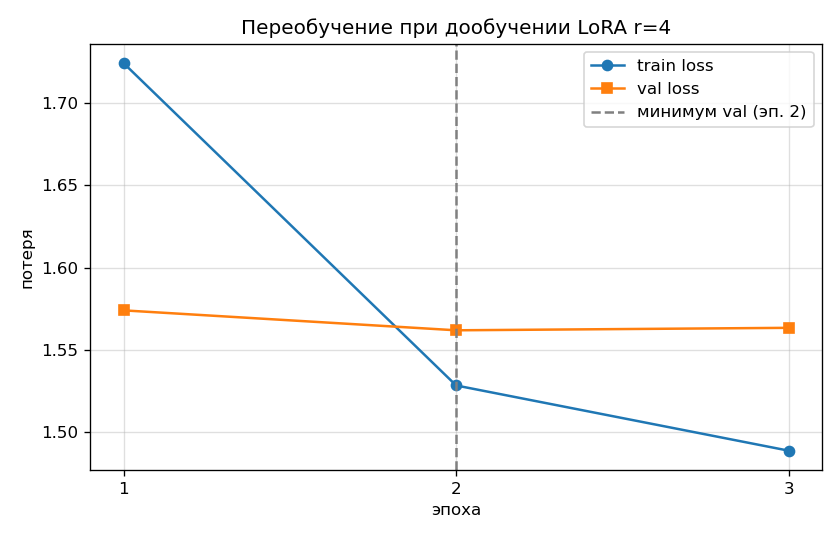
\includegraphics[width=0.72\textwidth]{overfit.png}
    \refstepcounter{figure}
    \caption*{Кривые train/val loss при дообучении LoRA $r=4$; пунктиром отмечен минимум val loss}
    \label{fig:overfit}
\end{figure}

Таблица трассировки ранней остановки (терпение 1 эпоха) приведена
в таблице~\ref{tab:early}.

\begin{table}[H]
    \centering
    \refstepcounter{table}
    \caption*{\raggedleft Трассировка ранней остановки (LoRA $r=4$)}
    \label{tab:early}
    \begin{tabular}{rrrrl}
        \toprule
        Эпоха & Val loss & Best & Wait & Действие \\
        \midrule
        1 & 1.5741 & 1.5741 & 0 & сохранить \\
        2 & 1.5620 & 1.5620 & 0 & сохранить \\
        3 & 1.5635 & 1.5620 & 1 & стоп (patience=1) \\
        \bottomrule
    \end{tabular}
\end{table}

\textbf{Шаг 3.2. Катастрофическое забывание.} Перплексия измерена на 50 отрезках
по 512 токенов тестового корпуса wikitext-2: у базовой модели (адаптер выключен)
PP $= 10.24$, у той же модели с обученным адаптером --- PP $= 10.13$, изменение
$-0.11$. Перплексия не выросла, а слегка упала: LoRA практически не ухудшила общие
знания базовой модели (в примере из методички полное дообучение давало рост 8.6
против 0.9 у LoRA --- у нас знак изменения благоприятный). Абсолютные значения
перплексии зависят от модели и корпуса, сравнивать нужно именно изменения.

\begin{table}[H]
    \centering
    \refstepcounter{table}
    \caption*{\raggedleft Сравнение метрик до и после дообучения LoRA ($r=4$)}
    \label{tab:forget}
    \begin{tabular}{lrrr}
        \toprule
        Метрика & База & После LoRA & Изменение \\
        \midrule
        BLEU на 50 тестовых примерах & 4.42 & 18.02 & $+13.60$ \\
        Перплексия wikitext-2 & 10.24 & 10.13 & $-0.11$ \\
        \bottomrule
    \end{tabular}
\end{table}

\textbf{Шаг 3.3. Память по правилу 18 байт на параметр.} При обучении со смешанной
точностью за каждый обучаемый параметр платится мастервес 4 Б + градиент 4 Б +
два момента Adam 8 Б + рабочий вес 2 Б = 18 Б. Полное дообучение всей модели
потребовало бы $1\,100\,048\,384 \times 18 \approx 18.4$ ГиБ --- это не помещается
ни в 6 ГиБ локальной видеокарты, ни в 16 ГиБ T4 без квантизации, что иллюстрирует
мотивацию метода LoRA. Для LoRA $r=4$ теоретическая память (обучаемые параметры
$\times$ 18 Б + хранение базы по 2 Б на параметр) $= 2.06$ ГиБ, фактический пик
\texttt{torch.cuda.max\_memory\_allocated()} при обучении --- 3.02 ГиБ
(таблица~\ref{tab:mem}). Расхождение $+0.96$ ГиБ объясняется активациями (даже с
gradient checkpointing), буферами смешанной точности и служебными структурами
тренера: правило 18 байт учитывает только веса и оптимизатор, но не активации.

\begin{table}[H]
    \centering
    \refstepcounter{table}
    \caption*{\raggedleft Оценка и факт потребления памяти}
    \label{tab:mem}
    \begin{tabular}{lrr}
        \toprule
        Способ дообучения & Теория, ГиБ & Факт (пик), ГиБ \\
        \midrule
        Полное дообучение & 18.4 & --- (не помещается) \\
        LoRA $r=4$ & 2.06 & 3.02 \\
        \bottomrule
    \end{tabular}
\end{table}

\textbf{Шаг 3.4. Влияние ранга (основной эксперимент).} Адаптеры обучены для всех
рангов ряда $\{4, 8, 16\}$ при одинаковых остальных настройках; результаты приведены
в таблице~\ref{tab:ranks} и на рисунке~\ref{fig:rank}. С увеличением ранга val loss
убывает почти незаметно ($1.5620 \to 1.5592$), а BLEU колеблется в пределах $\pm 0.2$
вокруг 18: разброс по всей таблице всего 0.41 пункта. \textbf{Точка насыщения
достигнута уже на самом маленьком ранге $r=4$}: четырёхкратное увеличение числа
параметров адаптера метрику задачи не улучшило, поэтому для этой задачи разумно
выбрать $r=4$ (минимум памяти и параметров при той же точности).

\begin{table}[H]
    \centering
    \refstepcounter{table}
    \caption*{\raggedleft Результаты дообучения по рангам LoRA}
    \label{tab:ranks}
    \begin{tabular}{rrrrr}
        \toprule
        Ранг & Параметры & Val loss & BLEU & Время, с \\
        \midrule
        4  & 563\,200   & 1.5620 & 18.02 & 4469 \\
        8  & 1\,126\,400 & 1.5594 & 17.87 & 4505 \\
        16 & 2\,252\,800 & 1.5592 & 18.28 & 4506 \\
        \bottomrule
    \end{tabular}
\end{table}

\begin{figure}[H]
    \centering
    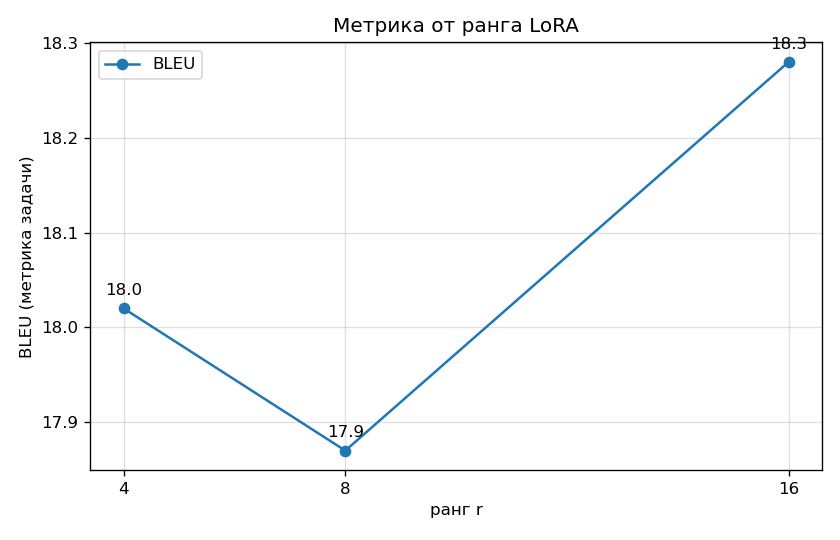
\includegraphics[width=0.72\textwidth]{rank_metric.png}
    \refstepcounter{figure}
    \caption*{Метрика BLEU от ранга адаптера LoRA}
    \label{fig:rank}
\end{figure}

\textbf{Шаг 3.5. Диагностика сбоев.} В таблице~\ref{tab:diag} отмечены симптомы,
которые наблюдались в экспериментах. Единственный отмеченный симптом --- «эхо
промпта» в 9 из 50 ответов после обучения: это в основном копирование служебных и
технических строк (маска при этом построена верно, \texttt{mt=1} стоит только на
токенах ответа); при необходимости данные стоит почистить. Остальные сбои
(переобучение, забывание, NaN, «двойной вывод») не наблюдались.

\begin{table}[H]
    \centering
    \refstepcounter{table}
    \caption*{\raggedleft Диагностика сбоев дообучения}
    \label{tab:diag}
    \small
    \begin{tabular}{p{0.24\textwidth}p{0.2\textwidth}p{0.24\textwidth}p{0.2\textwidth}}
        \toprule
        Симптом & Причина & Действие & Наблюдалось \\
        \midrule
        Модель повторяет промпт & маска не на ответе & \texttt{mt=1} только на токенах ответа &
        да (эхо 9/50 --- копирование служебных строк) \\
        train$\downarrow$, val$\uparrow$ со 2-й эпохи & переобучение & ранняя остановка, меньший $r$ & нет \\
        Старые умения пропали & полное дообучение без replay & replay 10--20\% старых данных, LoRA &
        нет (перплексия $-0.11$) \\
        Потеря не снижается & $B$ не нули, мала lr & проверить инициализацию и lr &
        нет (train снизился на 0.24) \\
        «Двойной» вывод после слияния & адаптер слит дважды & пересобрать из базовой модели &
        нет (слияние не выполнялось) \\
        NaN в потере & lr велика для fp16 & снизить lr, клиппинг градиента & нет \\
        \bottomrule
    \end{tabular}
\end{table}

\textbf{Вывод по заданию 3.} Переобучение при 1000 примерах только зарождается:
минимум val loss на 2-й эпохе, ранняя остановка останавливает обучение на 3-й.
Катастрофическое забывание отсутствует (перплексия $10.24 \to 10.13$), потребление
памяти LoRA (2.06 ГиБ по расчёту, 3.02 ГиБ факт) на порядок меньше требований полного
дообучения (18.4 ГиБ). Ранг работает как регуляризатор слабо: BLEU по рангам
4/8/16 практически одинаков (18.02/17.87/18.28), насыщение достигнуто при $r=4$.

\section{Вывод}

В ходе лабораторной работы выполнены все три задания варианта 16 (перевод EN$\to$DE
базовой моделью TinyLlama-1.1B-Chat и её дообучение LoRA). Установлено, что
детерминированные стратегии декодирования дают максимальные повторы и зацикливания,
сэмплирование --- галлюцинации на коротких входах; маска потерь устроена верно
(метки только на токенах ответа, сдвиг label shift на одну позицию учтён).
Ручной расчёт параметров адаптера LoRA (563\,200 при $r=4$, 0,051\% модели) сошёлся
с фактическим выводом \texttt{print\_trainable\_parameters}. Дообучение на 1000 пар
переводов повысило BLEU с 4.4 до 18.0 при обучении лишь 0,05--0,2\% параметров;
общие знания модели сохранены (перплексия wikitext-2 изменилась на $-0.11$),
потребление памяти снижено с теоретических 18.4 ГиБ полного дообучения до
фактических 3.02 ГиБ. Эксперимент с рангами показал, что насыщение метрики
достигается уже при $r=4$: для данной задачи и объёма данных более широкие
адаптеры не нужны.

\end{document}
